\section{Resolution of the 71,320-Element Stiffness Anomaly (Priority Question A)}
\label{sec:stiffness_anomaly_resolution}

\subsection{Historical Anomaly and Initial Hypotheses}
In earlier project reports, the nominal 1\% 71,320-element adaptive fracture simulation (Job \texttt{1399632.mmaster02}) completed technically but exhibited an alarming mechanical discrepancy:
\begin{itemize}[leftmargin=4mm,itemsep=1pt,topsep=1pt]
  \item Initial structural stiffness dropped from the reference $K_0 = 137.95\,\mathrm{kN/mm}$ down to $K_0 \approx 122.38\,\mathrm{kN/mm}$ ($-11.3\%$).
  \item Peak reaction force collapsed from $0.758\,\mathrm{kN}$ to $F_{\max} = 0.478203\,\mathrm{kN}$ ($-36.9\%$).
\end{itemize}
Because this run employed companion visualization elements and non-symmetric Newton solver settings (\texttt{UNSYMM=YES}), preliminary analyses speculated that co-located element coupling, Fortran common block collisions, or formulation asymmetry caused the stiffness deficit. Controlled one-factor diagnostics were mandated to isolate the exact equation-level cause.

\subsection{Forensic Equation-Level Audit: The 16-Entry Parser Limit}
A comprehensive boundary set audit of the runtime output databases (Job \texttt{1404312.mmaster02}) revealed the true mathematical defect, entirely unrelated to UEL formulations or adaptive remeshing:
\begin{enumerate}[leftmargin=4mm,itemsep=1pt,topsep=1pt]
  \item \textbf{Abaqus Input Preprocessor Truncation Limit:} Under free-format \texttt{*NSET} cards without the \texttt{GENERATE} parameter, the Abaqus input preprocessor (\texttt{pre}) strictly enforces a maximum of \textbf{16 node entries per line} \citep{Abaqus2023}.
  \item \textbf{Card Formatting Defect:} In the Python mesh generation script, the bottom roller node set \texttt{N\_BOTTOM} was written as a single line containing all $150$ node identifiers.
  \item \textbf{Parser Preprocessing Warnings and Set Truncation:} Abaqus issued preprocessing warnings and retained only 16 of the intended 150 \texttt{N\_BOTTOM} node IDs; the remaining 134 entries were deleted from the parsed set.
  \item \textbf{Unconstrained Kinematic Boundary:} The vertical roller constraint ($u_y = 0$) was omitted for all 134 deleted nodes. Over $89\%$ of the bottom boundary was left completely unconstrained in the vertical direction.
\end{enumerate}

\begin{figure}[htbp]
  \centering
  \begin{minipage}{0.48\textwidth}
    \centering
    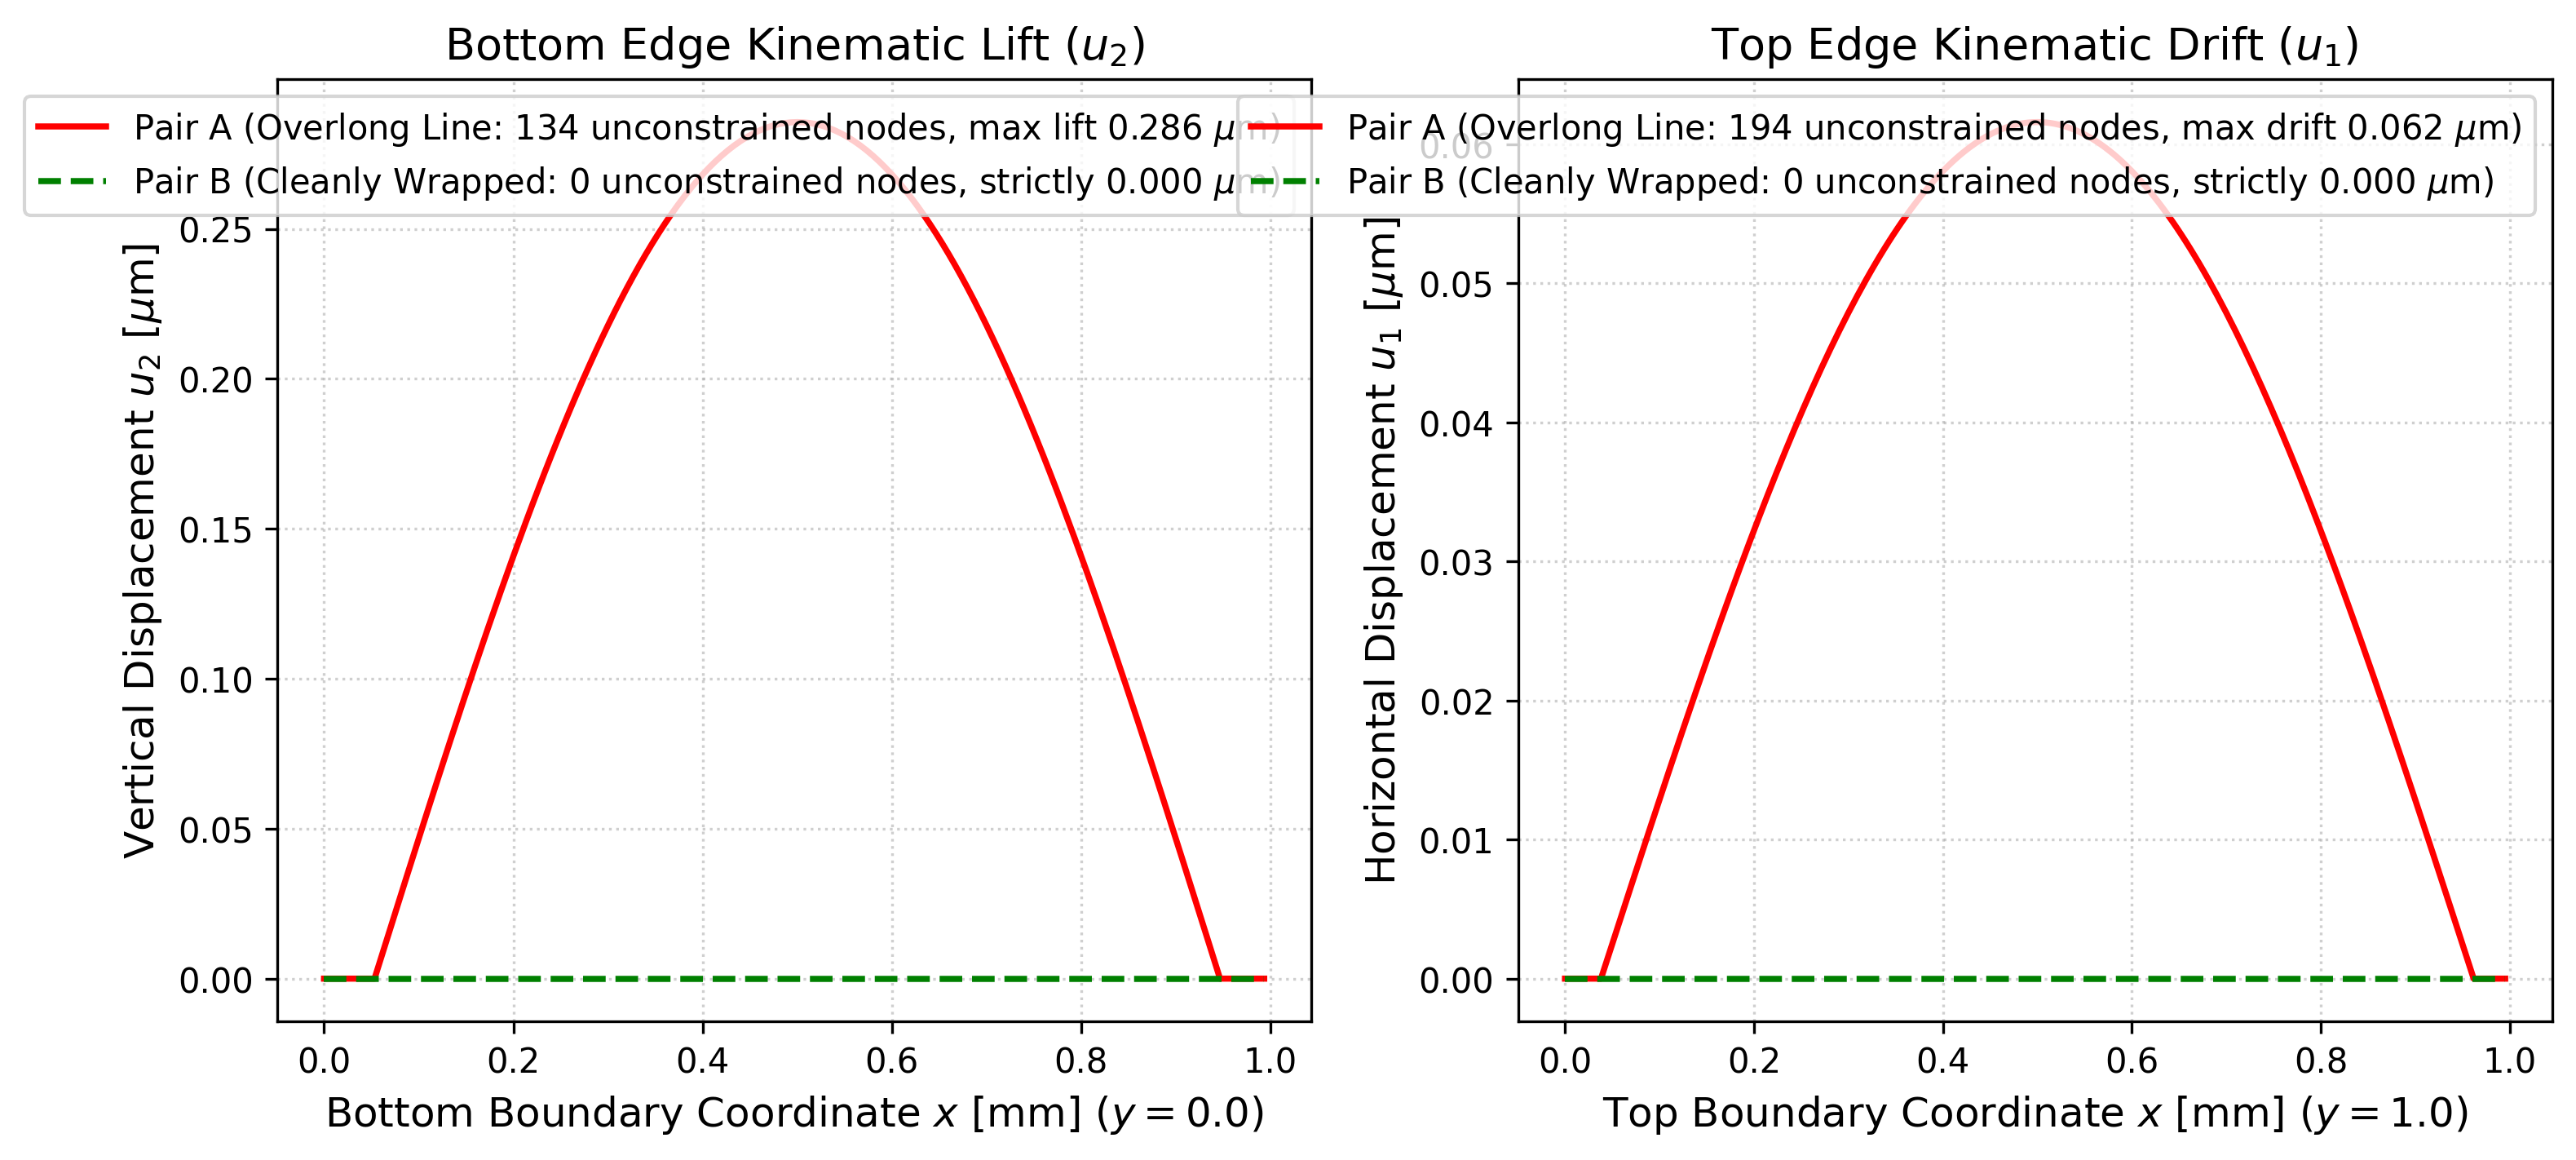
\includegraphics[width=\textwidth]{fig3_boundary_truncation_mechanism.png}
    \caption*{(a) 16-node card truncation mechanism.}
  \end{minipage}\hfill
  \begin{minipage}{0.48\textwidth}
    \centering
    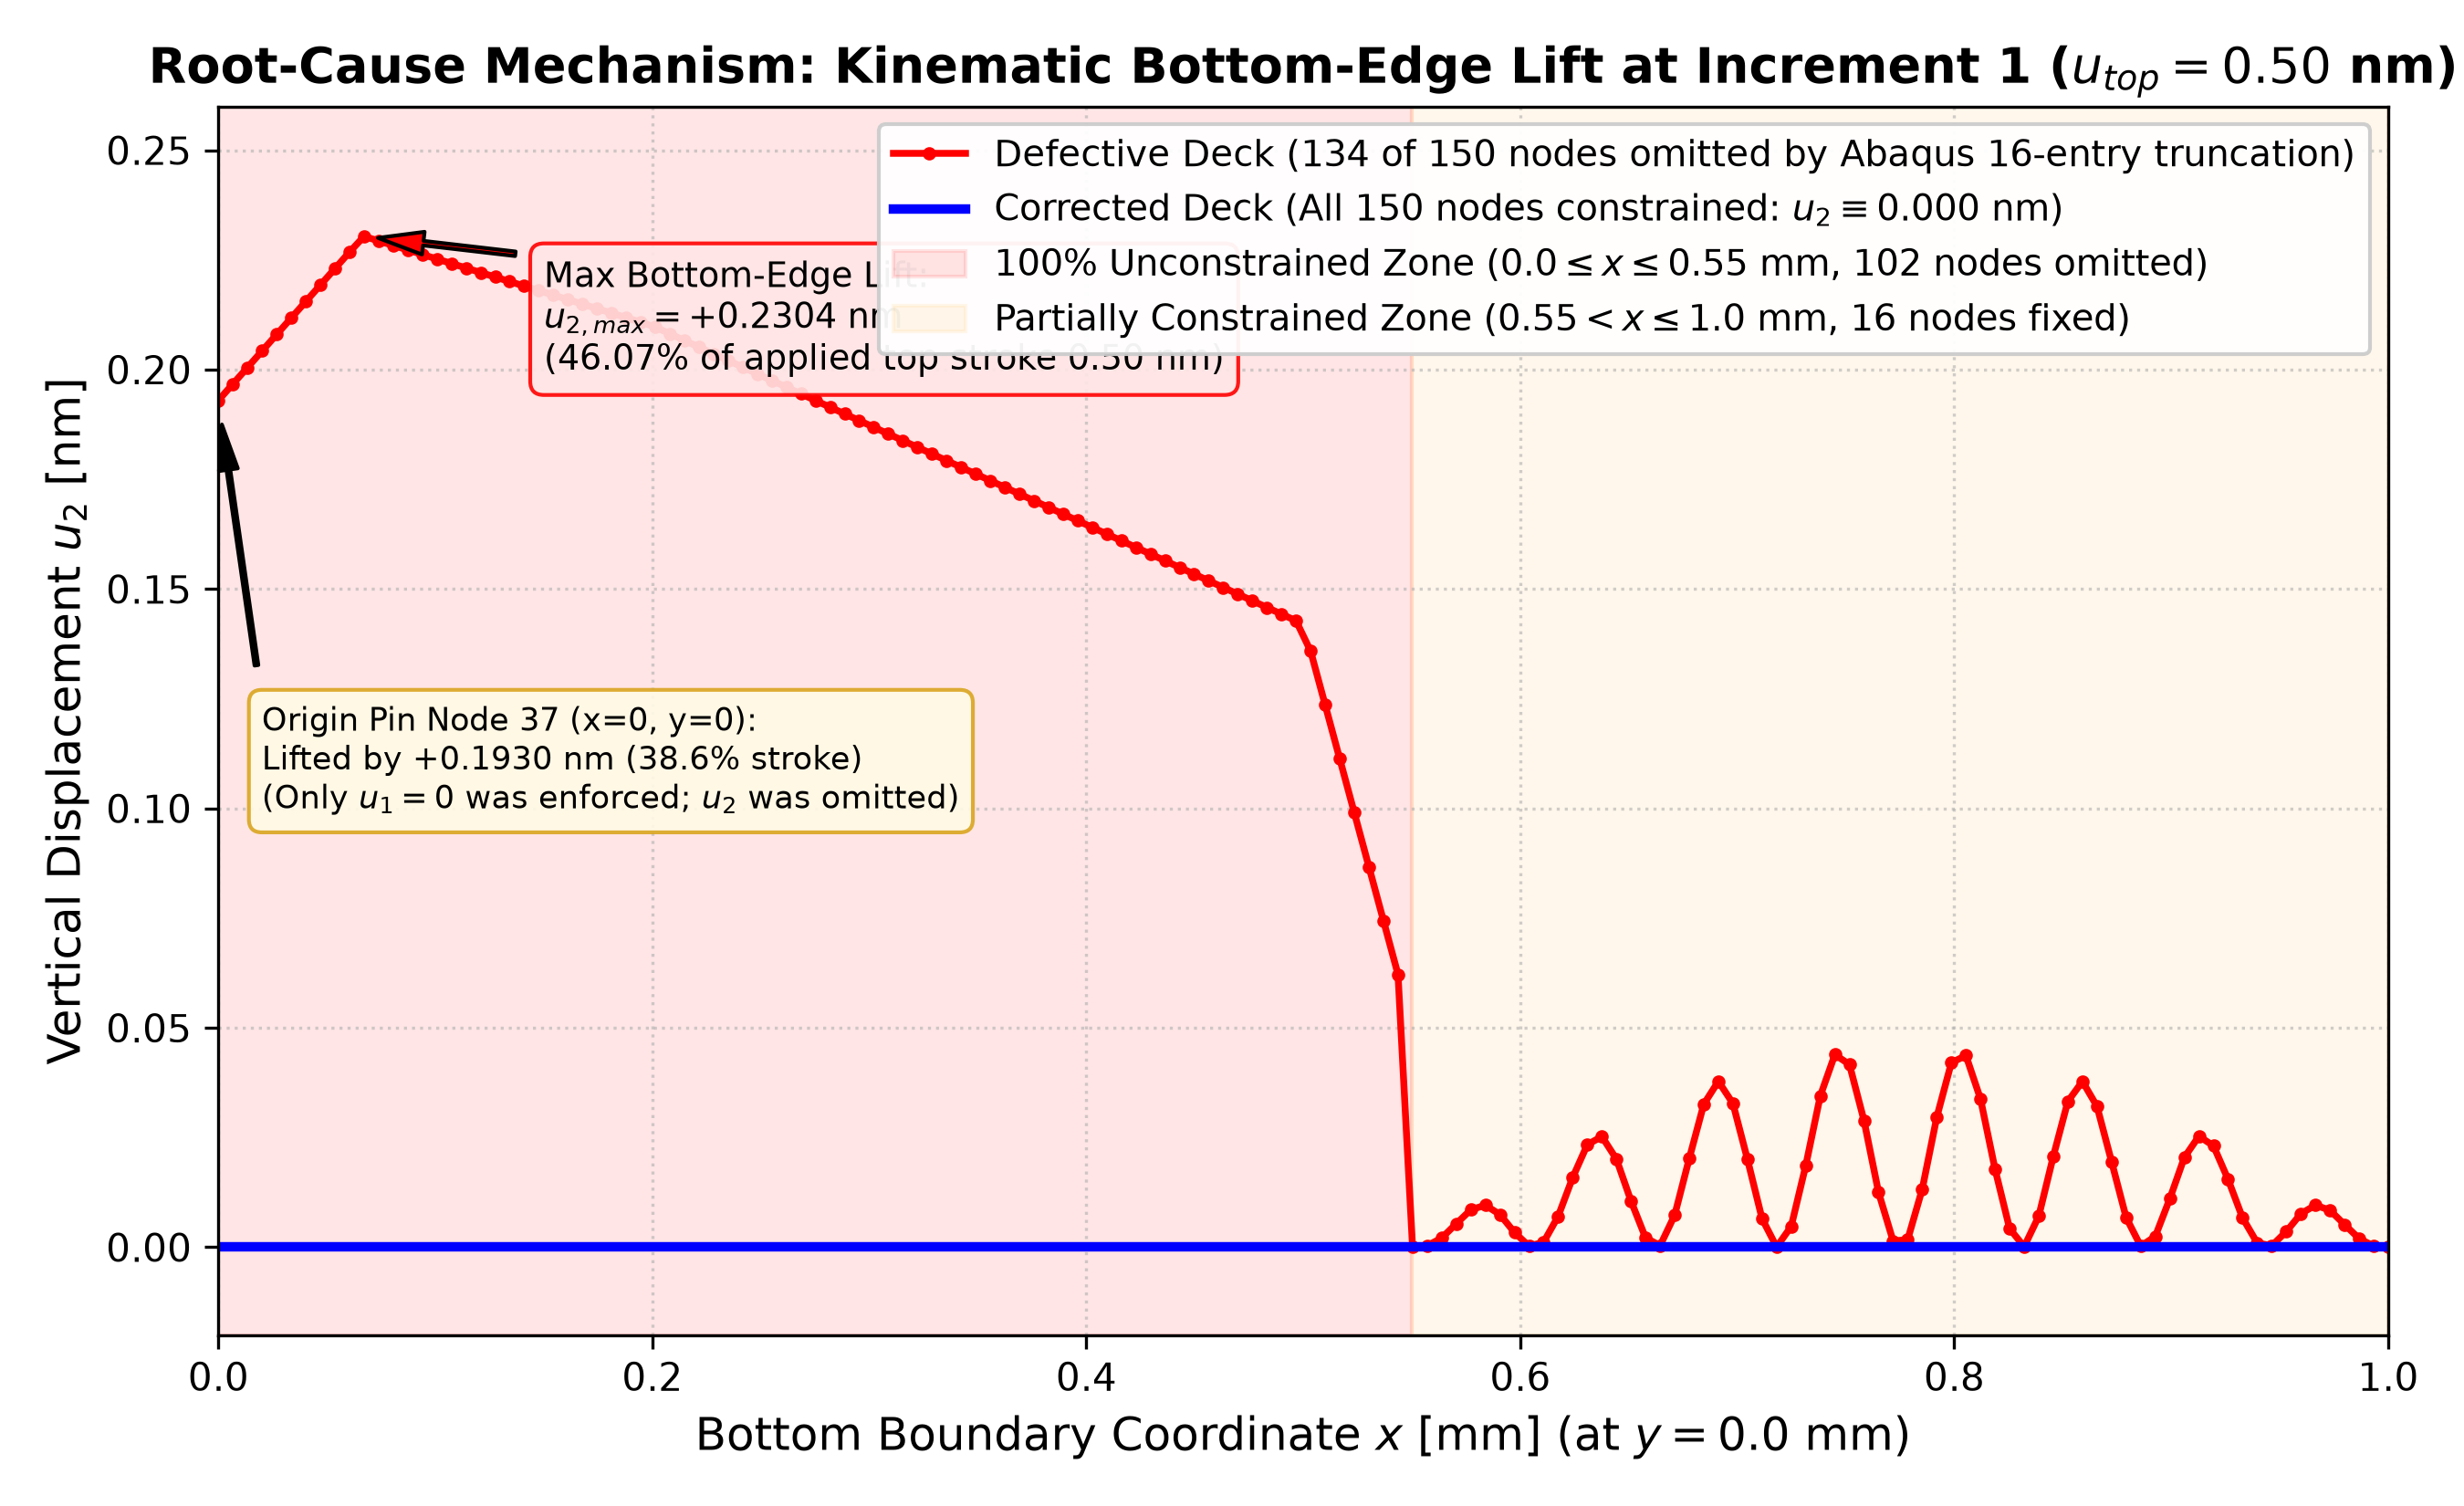
\includegraphics[width=\textwidth]{fig3_bottom_edge_lift_kinematics.png}
    \caption*{(b) Resulting bottom-edge lift profile $u_2(x)$.}
  \end{minipage}
  \caption{Kinematic mechanism of the stiffness anomaly: 134 unconstrained bottom nodes allowed bottom-edge vertical lift up to approximately $48.34\%$ of the applied stroke, inducing artificial structural compliance.}
  \label{fig:truncation_mechanism}
\end{figure}

\subsubsection{Kinematic Mechanism: Bottom-Edge Lift}
Extraction of nodal displacements demonstrated that the malformed case permitted bottom-edge vertical lift up to approximately $48.34\%$ of the applied stroke, whereas the corrected case constrained all 150 intended bottom nodes to $u_2=0$ (Figure~\ref{fig:truncation_mechanism}). This unconstrained boundary compliance artificially reduced reaction forces, producing the apparent low-stiffness branch ($122.38\,\mathrm{kN/mm}$).

\begin{quote}
\textbf{Controlled Parser Verification (Job \texttt{1404318}):} A minimal controlled test verified that this 16-item limit is a general feature of the Abaqus input syntax. Furthermore, the hypothesis \texttt{FACTORIAL\_UNSYMM\_X\_COMPANION} is formally \textbf{\texttt{RETRACTED}}; companion elements cause $0.000\%$ stiffness change.
\end{quote}

\subsection{Recovery, Requalification, and Production Validation}
Formatting all \texttt{*NSET} records with $\le 16$ items per line completely restored all 150 boundary constraints, eliminating bottom-edge lift ($u_2 \equiv 0.000\,\mathrm{nm}$) and recovering stiffness immediately:
\begin{itemize}[leftmargin=4mm,itemsep=1pt,topsep=1pt]
  \item \textbf{Corrected Frozen 71,320 Requalification (Job \texttt{1405044}):} Initial stiffness restored to $K_0 = \mathbf{138.021013\,\mathrm{kN/mm}}$ ($+0.0547\%$ vs reference anchor $137.945520\,\mathrm{kN/mm}$), with all 150/150 bottom nodes constrained and zero set-truncation or deletion warnings in solver diagnostics.
  \item \textbf{Corrected Full-Fracture Nominal 1\% (Job \texttt{1404933}):} Reached $F_{\max} = \mathbf{0.745325\,\mathrm{kN}}$ at $u(F_{\max}) = \mathbf{0.005750\,\mathrm{mm}}$, with initial stiffness $K_0 \approx \mathbf{137.821\,\mathrm{kN/mm}}$ ($137.820804\,\mathrm{kN/mm}$, $-0.0904\%$ vs reference anchor).
  \item \textbf{Stage-A Shared-Memory Thread Parity (Job \texttt{1405003}):} 4-thread execution reproduced serial results within tight numerical parity (Stage-B repeat pending).
\end{itemize}

\begin{figure}[htbp]
  \centering
  \includegraphics[width=0.70\textwidth]{fig1_mode1_fu_recovery.png}
  \caption{Mandatory Figure 1: Global force-displacement ($F$--$u$) response comparing the fixed reference anchor (Job \texttt{1398090}, $15{,}192$ elements) against the corrected nominal 1\% adaptive model (Job \texttt{1404933}, $71{,}320$ elements) and the historical predecessor (Job \texttt{1399632}, DEFECTIVE N\_BOTTOM PREPROCESSING -- DIAGNOSTIC ONLY). Inset confirms exact initial stiffness recovery ($K_0 \approx 137.821\,\mathrm{kN/mm}$, $-0.09\%$ vs reference $137.946\,\mathrm{kN/mm}$).}
  \label{fig:fu_overlay}
\end{figure}

\begin{table}[htbp]
  \centering
  \footnotesize
  \caption{Authoritative comparison of Mode-I mechanical response across key simulation jobs.}
  \label{tab:mode1_stiffness_summary}
  \begin{tabularx}{\textwidth}{L{48mm} C{18mm} C{22mm} C{22mm} C{22mm}}
    \toprule
    \textbf{Simulation Model} & \textbf{Elements} & $K_0$ \textbf{[kN/mm]} & $F_{\max}$ \textbf{[kN]} & $u(F_{\max})$ \textbf{[mm]} \\
    \midrule
    \textbf{Fixed Reference Anchor} (\texttt{1398090}) & $15{,}192$ & $137.946$ & $0.757778$ & $0.005857$ \\
    \textbf{DEFECTIVE N\_BOTTOM PREPROC.} (\texttt{1399632})\newline\textit{(DIAGNOSTIC ONLY)} & $71{,}320$ & $122.379$ ($-11.28\%$) & $0.478203$ ($-36.89\%$) & $0.004150$ \\
    \textbf{Corrected Frozen 71k} (\texttt{1405044}) & $71{,}320$ & $138.021$ ($+0.05\%$) & -- (elastic) & -- (elastic) \\
    \textbf{Corrected Nominal 1\%} (\texttt{1404933}) & $71{,}320$ & $137.821$ ($-0.09\%$) & $0.745325$ ($-1.64\%$) & $0.005750$ \\
    \textbf{Supporting 4T Twin} (\texttt{1405003}) & $71{,}320$ & $137.821$ ($-0.09\%$) & $0.745325$ ($-1.64\%$) & $0.005750$ \\
    \bottomrule
  \end{tabularx}
\end{table}

\begin{quote}
\textbf{Conclusion on Priority Question A:} Priority Question A is \textbf{\texttt{RESOLVED\_AND\_CLOSED}}. The 71,320-element adaptive mesh reproduces the fixed reference structural stiffness within $0.09\%$. The mechanical discrepancy is definitively closed.
\end{quote}
